%% статьи в формате LaTeX для сборника статей "Системное         **
%% **  программирование".                                                   **
%% **  СПбГУ, мат.-мех. факультет, НИИ ИТ, 2005 г.                          **
%% **  Текст собирается с помощью программы latex                           **
%% **                                                                       **
%% ***************************************************************************

\documentclass[a5paper]{article}
\usepackage[a5paper, top=17mm, bottom=17mm, left=17mm, right=17mm]{geometry}
\usepackage[T2A]{fontenc} 
\usepackage[utf8]{inputenc}
\usepackage[english,russian]{babel}
\usepackage{graphicx}
\usepackage{indentfirst}
\usepackage{hyperref}
\usepackage{textcomp}
\usepackage{amsthm}


\sloppy
\pagestyle{empty}

%% ***************************************************************************
%% **                                                                       **
%% **  Место для названия статьи                                            **
%% **                                                                       **
%% ***************************************************************************
\title{Формальные языки}

%% ***************************************************************************
%% **                                                                       **
%% **  Место для авторов, их email-адресов и названий институтов            **
%% **                                                                       **
%% ***************************************************************************
%\author{С.В.Григорьев\\
%rsdpisuy@gmail.com\\
%\and Санкт-Петербургский государственный университет\\
%198504, Университетский проспект, 28, Старый Петергоф,\\
%Санкт-Петербург, Россия}
%\date{}
\begin{document}

\theoremstyle{definition}
\newtheorem{mydef}{Definition}
\newtheorem{mytheorem}{Theorem}


%\maketitle
%\thispagestyle{empty}

%% ***************************************************************************
%% **                                                                       **
%% ** Аннотация                                                             **
%% **                                                                       **
%% ***************************************************************************
%\begin{quote}

%\renewcommand{\thefootnote}{}

%% ***************************************************************************
%% **                                                                       **
%% ** Авторские права                                                       **
%% **                                                                       **
%% ***************************************************************************
%\setcounter{footnote}{0}
%\end{quote}

%% ***************************************************************************
%% **                                                                       **
%% ** Текст статьи                                                          **
%% **                                                                       **
%% ***************************************************************************
\section{Краткре содержание}

\begin{itemize}
    \item Введение. Алфавит, слово, язык.
    \item Способы задания языка: порождение, генерация, грамматика, уравнения, логика над позициями.
    \item Грамматика, вывод, дерево вывода, однозначные, неоднозначные языки и грамматики
    \item Конъюнктивные языки, грамматики. Булевы языки, грамматики.
    \item нормальная форма Хомского 
    \item CYK
    \item Синтаксический анализ графов
    \item Перемножение матриц, алгоритм Уоршалла
    \item LL, FIRST, FOLLOW, устранение левой рекурсии, левая факторизация, не LL языки
    \item GLL, поддержка EBNF, поддержка нелинейного входа
    \item Tree languages, SPPF --- regular tree language
    \item Почему работает синтаксический анализ графов
    \item PEG
    \item комбинаторы
\end{itemize}


\section{Лекция 1. Введение}
\subsection{Алфавит, слово, язык}

\subsection{Способы задания языка}


\section{Лекция 2. Грамматика, вывод}
\subsection{!!!}

\subsection{Способы задания языка}

\section{Лекция k. Tree languages}

Вспомним определение языка. Вообще говоря, мы просто описываем правила построения некоторых множеств. Давайте констуировать множества деревьев.

Давайте взглянем на CYK. На тот CYK, который умеет строить деревья. Или просто на правила построения деревьев вывода. Вообще говоря, если не разделять шаги, то мы можем строить множества деревьев по каким-то правилам.

Эти множества могут обладать некоторыми интересными свойствами и их можно изучать как обобщённые структуры, а не страдать с каждым деревом отдельно. Вы наверняка знаете про бинарные деревья, вообще n-арные, сбалансированные и т.д.
\begin{mydef}[Tree grammar]
Tree grammar $G=(S,N,F,P)$
\begin{itemize}
\item $S$ --- аксиома. Сартовый нетерминал.
\item $N$ --- нетерминальные символы
\item $F$ --- терминальные символы
\item $P$ --- продукции вида $ \alpha \rightarrow \beta $ $\alpha, \beta$ --- деревья.
\end{itemize}
\end{mydef}

Грамматика над деревьями называется регулярной, если все нетерминальные символы имеют арность 0, и все продукции имеют вид $A \rightarrow \beta, A \in N, \beta is T(F \cup N)$


Пример --- списки натуральных чисел.


\begin{mytheorem}
\begin{enumerate}
\item $G$ --- CF grammar, тогда множество всех деревьев разбора $L(G)$ --- регулярный язык деревьев.
\item $L$ --- регулярный язык деревьев, тогда $Yield(L)$ --- контекстно свободный язык.
\item Существуют регулярные языки деревьев, не являющиеся множеством деревьев вывода никакого плоского КС.
\end{enumerate}
\end{mytheorem}

Пункт 1. $G=(S,N,\Sigma,P)$ --- КС грамматика. $G'=(S,N,F,P')$ --- регулярная грамматика деревьев.

\begin{itemize}
\item $F=\Sigma \cup \{\varepsilon\} \cup \{A_n | A \in N, \exists A \rightarrow \alpha \in P, |\alpha| = n\}$
\item Если $(A \rightarrow \varepsilon) \in P$, тогда $A \rightarrow A_0(\varepsilon) \in P'$
\item Если $(A \rightarrow a_1 \dots a_p) \in P$, тогда $A \rightarrow A_p(a_1, \dots, a_p) \in P'$
\end{itemize}


Интересен пункт 3.

$G=(S,N,F,P), F =(s(,); g(); a; b), N=(S;G';G''), P = (S \rightarrow s(G',G'');G' \rightarrow g(a); G'' \rightarrow g(b))$
В $L(G)$ есть единственное дерево $s(g(a),g(b))$.

Если попробуем построить КС-грамматику, то получим что-то вроде S->GG, G->a, G->b. В таком языке есть "aa" -> S(G(a),G(a))

%\begin{figure}
%    \begin{center}
%        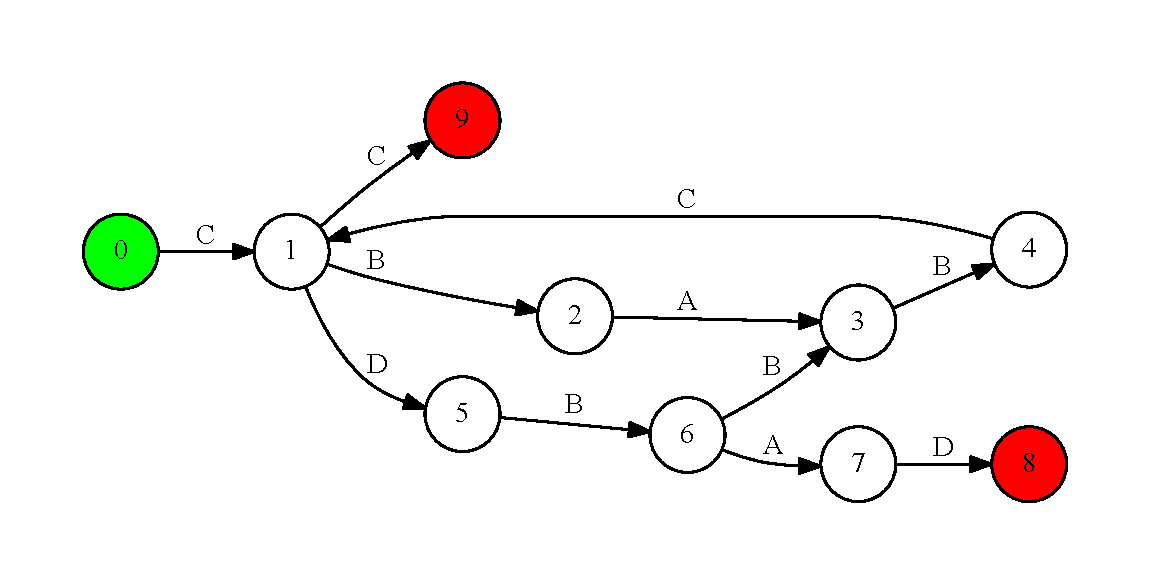
\includegraphics[width=11cm]{input.pdf}
%        \caption{Входной граф}
%        \label{pic1}        
%    \end{center}
%\end{figure}
%


%% ***************************************************************************
%% **                                                                       **
%% ** Список литературы                                                     **
%% **                                                                       **
%% ***************************************************************************
\begin{thebibliography}{99}
  
\bibitem{SCFGRNA1}
Dowell R. D., Eddy S. R. Evaluation of several lightweight stochastic context-free grammars for RNA 
secondary structure prediction //BMC bioinformatics. --- 2004. --- Т. 5. --- \textnumero. 1. --- С. 1.

\bibitem{SCFGRNA2}
Eddy S. R. A memory-efficient dynamic programming algorithm for optimal alignment of a sequence to 
an RNA secondary structure //BMC bioinformatics. --- 2002. --- Т. 3. --- \textnumero. 1. --- С. 1.

\bibitem{STEMSEARCH1}
Yogev S., Milo N., Ziv-Ukelson M. StemSearch: RNA search tool based on stem identification and indexing //Bioinformatics and Biomedicine (BIBM), 2013 IEEE International Conference on. --- IEEE, 2013. --- С. 145-152.

\bibitem{STEMSEARCH2}
Eddy S. R. Homology searches for structural RNAs: from proof of principle to practical use //RNA. --- 2015. --- Т. 21. --- \textnumero. 4. --- С. 605-607.

\bibitem{SCFGHARD1}
Anderson J. W. J. et al. Evolving stochastic context--free grammars for RNA secondary structure prediction //BMC bioinformatics. --- 2012. --- Т. 13. --- \textnumero. 1. --- С. 78.



\end{thebibliography}

\end{document}
